\section{評価の方法}
\label{sec_exp}
\begin{figure*}[t]
    \centering
    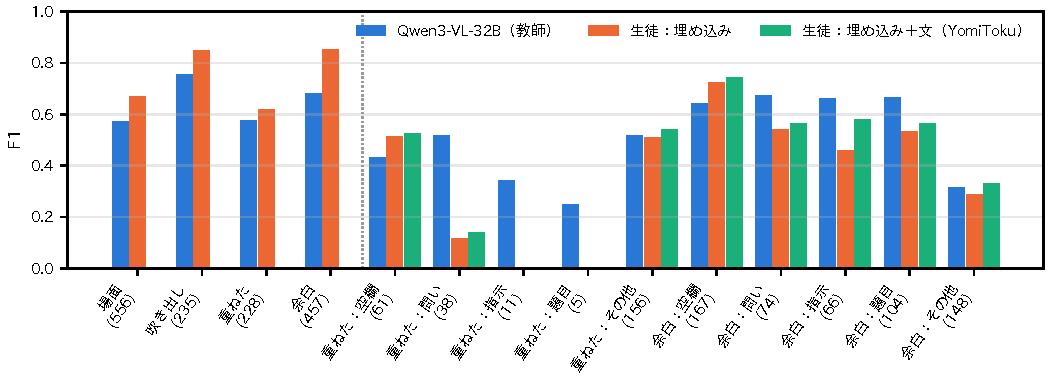
\includegraphics[width=\textwidth]{figures/fig_attrs.pdf}
    \caption{属性ごとの F1（1,620枚）．生徒は5分割の交差検証の分割外の予測であり，層の属性は埋め込みのみで学習した}
    \label{fig_attrs}
\end{figure*}

\subsection{目視ラベル}
\ref{sec_intent}章の1,020枚と600枚を合わせた1,620枚に，提案の属性の目視ラベルを付けた．
画像は並べ替えて番号だけを付けた一覧の画像にし，パッケージの予測と第5版の目視ラベルを伏せて付与した．
再現性を確かめるため，1,620枚から無作為に選んだ90枚を番号を付け直して別の一覧にし，同じ判断者が付け直した．
全データの推定値は，600枚に(\ref{eq_weighted_pr})の重みを用いて求め，1,020枚は学習と重みなしの値にのみ用いた．
2つのラベルの一致は，重み付きの一致率と Cohen の $ \kappa $ で評価した．

\subsection{教師}
教師は Qwen3-VL-32B-Instruct の FP8 量子化版であり，入力の画素数の上限は802,816画素である．
4つの層の有無，重ねた文字と余白の文字の文の形，両層の書き起こしを JSON の形式で答えさせた．
また，書き起こしだけを答えさせる指示を，同じモデルと Qwen3-VL-2B-Instruct に問うた．
YomiToku でも全ての文字を書き起こしたが，YomiToku は層を区別しない．

\subsection{生徒}
生徒は，属性ごとのロジスティック回帰であり，1,620枚の5分割の交差検証で分割外の予測を求めた．
入力は，パッケージが保存した SigLIP 2 の1,152次元の画像埋め込みと，書き起こした文の文字の1〜3-gram の Term Frequency-Inverse Document Frequency (TF-IDF) の特徴である．
文の特徴は，教師の書き起こしでは重ねた文字と余白の文字を別の語彙とし，YomiToku の書き起こしでは全ての文字を1つの語彙とした．
層の属性は埋め込みだけで学習し，文の形の属性は埋め込み，文，両方の3通りで学習した．
正則化の係数は，埋め込みで $ C = 0.05 $，文で $ C = 4 $，両方で $ C = 1 $ とし，正例と負例の重みを釣り合わせた．
確率が0.5以上の場合に真とした．

お題文ありの予測は2通りで求めた．
1つ目は，生徒の層と形の予測を(\ref{eq_rules})に代入して導く方法である．
2つ目は，規則で導いた目視のお題文ありを，属性を経ずに直接学習する方法である．
比較の基準は，第5版の定義で学習したパッケージ v5.3.0 のお題文ありである．
パッケージの生徒は約4.5万枚の教師ラベルで学習しており，1,620枚で学習した生徒とは学習の量が異なる．
